%% Nemanja Milosevicr
%% phd text

%% feel free to reuse parts (or all) of the formating
%% in other words the Latex code can be used as Public Domain

%% The text itself is released under a CC-BY-SA 4.0 licence

%% Most of the code presented can be found under a GPL licence

\documentclass[b5paper]{book}

%custom packages
\usepackage[T1]{fontenc}
\usepackage[utf8]{inputenc}
\usepackage[serbian,english]{babel}

\usepackage[autostyle=true]{csquotes}
\DeclareQuoteAlias{croatian}{serbian}

% needs this declaration for ayodeji
\DeclareUnicodeCharacter{1ECD}{\d o}

%change the default font
\usepackage{lmodern}
\usepackage{nimbusmono}
\renewcommand{\familydefault}{\sfdefault}

\usepackage{ccicons}

\usepackage{ctable}
\usepackage{wrapfig}

\newcommand{\autor}{Nemanja Milošević}
\newcommand{\autorkratko}{N.-Milošević}
\newcommand{\naslov}{Negative Deep Learning}
\newcommand{\naslovsr}{Negativno duboko učenje}

\usepackage[style=authoryear-comp,sorting=nyt,maxnames=4,backend=biber,backref=true,natbib]{biblatex}

\AtEveryCite{%
  \let\parentext=\parentexttrack%
  \let\bibopenparen=\bibopenbracket%
  \let\bibcloseparen=\bibclosebracket}

\addbibresource{references.bib}

% use parens for cite

\let\oldcite\cite
\let\cite\parencite


% pdf export settings
\usepackage[%
%colorlinks,
bookmarksopen,bookmarksnumbered,citecolor=red,
%urlcolor=red,
pdffitwindow=false,unicode=true,%
pdftitle={\naslov},%
pdfauthor={\autor}%
]{hyperref}

\usepackage{graphicx}
\usepackage{fancyhdr}

\fancypagestyle{plain}{%
\fancyhead{} % get rid of headers on plain pages
\fancyfoot{}
\renewcommand{\headrulewidth}{0pt} % no lines
\renewcommand{\footrulewidth}{0pt} % 
}

% empty pages, really empty
\makeatletter
\def\cleardoublepage{\clearpage\if@twoside \ifodd\c@page\else
\hbox{}
%\vspace*{\fill}
%\begin{center}
%This page intentionally contains only this sentence.
%\end{center}
%\vspace{\fill}
\thispagestyle{empty}
\newpage
\if@twocolumn\hbox{}\newpage\fi\fi\fi}
\makeatother

% put figures in the figures folder
\graphicspath{{./figures/}}

\usepackage[figure,table,page]{totalcount}

\newcounter{citenum}
\AtEveryBibitem{\stepcounter{citenum}}

\usepackage{amsthm}
\usepackage{amsmath}
\usepackage{latexsym}

\usepackage{listings}

% if we want to make an index at the end we need this
% this document didn't have an index in the end
%\usepackage{makeidx}

%\makeindex

\lstset{
        basicstyle=\small\ttfamily,
        showstringspaces=false,
        breaklines=true
}

\lstloadlanguages{Python}

\lstnewenvironment{codeblock}
{\lstset{basicstyle=\footnotesize\ttfamily,
        columns=fixed}}
{}

%options to the lst can be given through this
\lstnewenvironment{codeblock1}[1]
{\lstset{basicstyle=\footnotesize\ttfamily,#1,
        columns=fixed}}
{}

\lstnewenvironment{codeblockw}
{\lstset{basicstyle=\footnotesize\ttfamily,
    language=wsl,
        columns=fixed}}
{}
\lstnewenvironment{codeblocka}
{\lstset{basicstyle=\footnotesize\ttfamily,
    language=[x86masm]Assembler,
        columns=fixed}}
{}
\lstdefinestyle{asmblock}{
  language=[x86masm]Assembler,
  basicstyle=\footnotesize\ttfamily
}
\lstdefinestyle{codeblock}{
        basicstyle=\footnotesize\ttfamily,
        columns=fixed,
        language=wsl
}

\lstdefinestyle{codeblockb}{
        basicstyle=\normalsize\ttfamily,
        columns=fixed,
        language=wsl
}


%% `skica' is Serbian for `sketch', these blocks were used in the development
%% of the document for various reminders

% skica can take a normal paragraph and present it more or less as such
\newcommand{\skica}[1]{
    \noindent \framebox{\parbox[c]{0.9\textwidth}{  {\small** {#1}  }}
    \newline }
}

% skicas is a small sketch, intended mostly for inline use
\newcommand{\skicas}[1]{
    \framebox{* \small \textit{#1} *}
}

% b is for bold sketches, things that are high priority
\newcommand{\skicab}[1]{
  \noindent \framebox{\parbox[c]{0.9\textwidth}{ {\small***
        \textbf{#1} }} \newline } }

% special words inline such as class and method names
%\newcommand{\kod}[1]{{\small\texttt{#1}}}
\newcommand{\kod}[1]{\lstinline[]`#1`}
\newcommand{\code}[1]{\lstinline[]`#1`}
\newcommand{\codea}[1]{\lstinline[style=asmblock]`#1`}
\newcommand{\codew}[1]{\lstinline[style=codeblock]`#1`}

%% these commands were used to get a clean version of the text
%% without the sketches

%\renewcommand{\skica}[1]{}
%\renewcommand{\skicas}[1]{}


% experimental, for one line of par being split over a page
\widowpenalty=10000
\clubpenalty=10000

% ----------------===========--------------------------------------
%                 start paper


\author{\autor}
\title{\naslov}
\date{Novi Sad, 2020}
\begin{document}
\frontmatter

\newcommand{\makemytitle}{
  \begin{center}

	
\includegraphics[width=1.8cm]{pmf-logo}\hspace{\stretch{1}}
	\parbox[b]{45ex}{\centering
          University of Novi Sad\\
Faculty of Sciences\\
Department of Mathematics and Informatics\\ }\hspace{\stretch{1}}
	
\includegraphics[width=1.8cm]{uns-logo}

	\vspace{15ex}

	\parbox[b]{\textwidth}{{\Large {\bf \hspace{0.5cm}Nemanja Milošević}}}
	\vspace{4ex}

	{\huge
            \setlength{\baselineskip}{1.5\baselineskip}\textbf{\naslov}\par}

	\vspace{4ex}
	-- Doctoral dissertation  --

        \vspace{5ex}

	{\huge
            \setlength{\baselineskip}{1.5\baselineskip}\textbf{\naslovsr}\par}

	\vspace{4ex}
	-- Doktorska disertacija  --

	\vfill

	Novi Sad, 2020
	\end{center}
	\thispagestyle{empty}
	\newpage
}

\makemytitle

~

\vfill

\thispagestyle{empty}
\noindent CC BY-SA \ccbysa\\
\textcopyright \ 2020 Nemanja Milošević\\
This work is licensed under a
Creative Commons Attribution Share Alike 4.0 International Licence
\url{https://creativecommons.org/licenses/by-sa/4.0/}

\chapter{Preface}
\chapter{Abstract}

\tableofcontents

\mainmatter

\part{Introduction}

In the first part of this dissertation a short history of the field is presented with focus on some models and approaches used later to define and describe negative deep learning models. 

\chapter{Artificial Intelligence: A brief overview}

Artificial intelligence is an universal field. Whether it is writing poetry, playing chess, proving theorems, self-driving cars or any other intellectual task, throughout history scientists have tried different artificial intelligence (AI) methods to bring the machines closer to us humans. Even though we think AI is the "new and hot" field in Computer Science, modern AI roots can be traced all the way to World War II. The name was coined after (in 1956) but the science was there long before that. From Alan Turing to Yann LeCun and others, generations have been working hard to bring the dream closer to reality -- a dream where machines can think, and reason. From the iconic Turing test to the deep neural networks, we have come long way but we still have loads to discover.

\section{History of Artificial Intelligence}

Many have tried to precisely define what AI means. Today, we know that a single, all encompassing definition is very difficult to formulate. AI is concerned with reasoning, behaviour, thought process, rational thinking and other well-defined terms. Therefore we define AI as a sum of everything that makes machines perform closely to human level. In other words machines need to learn to do the "right thing", given the knowledge we possess.

@@@ IAN
In the early days of AI, researchers sought ways to solve difficult problems for humans. These problems proved to be easy for machines to comprehend through a series of formal, mathematical rules. The real challenge today is solving the tasks that easy for humans but hard to describe formally -- problems that feel automatic, intuitive like recognizing spoken words or faces in images.

To try and provide the scientific world with an operational definition of intelligence, Alan Turing (1950) devised the famous Turing Test. A machine (in other words software) passes the test if a human asking series of questions cannon tell whether the responses are coming from a person or a computer. To develop software able to do this is not an easy task. The system would have to have many capabilities including: natural language processing (so it can communicate), knowledge representation (so it can store what it knows), automated reasoning (to draw conclusions from the knowledge) and machine learning (to adapt to new environments and detect and understand patterns in knowledge). In addition to these capabilities if we were not to avoid human-machine physical contact, the machine would also have to be able to see (computer vision) and interact with the real physical world (robotics). The six capabilities remain relevant today, 70 years after the Turing Test was formulated.

Today, researchers are not pursuing the solution to the Turing Test actively as before. The reason in in believing that it is more important to study the underlying principles of intelligence, than to duplicate it. 

With that in mind, comes the state-of-art-approach as of today -- Deep Learning.

Our "seat of consciousness", the brain, is the main object of study in neuroscience. Even though even today, the exact way in which the brain functions remains one of the great (if not the greatest) mysteries of science, the simple fact that it does enables the drive of researchers to push further and further in the quest of fully understanding the how and the why. In the 18th century, humanity was certain that the brain is the center of reason in humans, and in the 19th century we were made aware the brain contains many neurological cells called neurons. (Golgi, Broca) In the early 20th century, Nicolas Rashevsky was the first to apply mathematical models in studying the nervous system. 

Neurons or nerve cells are built from two major parts: cell body (soma) which contains a cell nucleus and a number of fibers called dendrites on of which is longer than the others (axon). Axon length is particularly interesting, some can be up to a meter long. A typical biological neuron makes connections with 10 to 100000 other neurons at junctions which are called synapses. Signals are propagated though neurons by the means of a complicated electrochemical reaction. The signals are used to control brain activity but can also enable long-term changes in connections between neurons. We believe that these mechanisms enable our brains to learn. It is amazing to think that a structure of simple cells can lead to thoughts or that in other words: brains cause minds (John Searle, 1992).

\section{Reappearance of Neural Networks with modern hardware development}

With modern GPU (graphical processor unit) development, especially the developments related to the NVIDIA CUDA framework, deep neural network models were suddenly possible and obtainable.

The human brain consists of around 100000000000 neurons (10\^11). A modern computer can have even more transistors, thus we are approaching singularity -- a point in time where computers reach superhuman levels of performance. The raw comparison is not especially informative (or right) since that even if one made a computer with unlimited resources and capabilities, we still would not know how to achieve brain's level of intelligence.

In the mid 1980s at least four different research groups revisited backpropagation learning algorithm developed 20 years earlier by Bryson and Ho. The so called connectionist model was seen by some as a direct competitor to previously developed symbolic models and also to the logicist approach. The current view is that all these approaches are complementary, not excluding.

\section{Modern Machine Learning}

As algorithms developed and we learned more and more about intelligence, one thing was very clear: AI systems must have the ability to acquire their own knowledge. This is done by extracting knowledge (patterns) from raw data. The performance of the system still relies heavily on the operator in crucial way and that is the was the data is represented. This is why almost all algorithms require specific data presented in a specific way in order to be useful. Each piece (called feature) of information can be very important. Machine learning algorithm outcome is influenced by the feature values, in other words the algorithm learns to correlate these feature values and the outcome values.

In many tasks it is very difficult to define data structures in a way that it is easy to extract meaningful feature values. This is why researchers rely on fields like representation learning where the algorithm is forced to not only provide some reasoning or outcome of the feature value inputs but also a different, more efficient representation of the input features. These representations can be very complex and difficult to interpret and that is why today we rely on stacking many simplified versions of them. If we were to draw the structure of these algorithms we would need a lot of space, because we can make them very deep. So deep in fact that they are called: Deep Learning algorithms.

\section{Deep Learning and its common uses}

Deep Learning uses stacked feature representations to define complex relationships between input patterns and output data. With Deep Learning, we can build complex concepts out of simpler concepts, and that is a very powerful paradigm. 

The simplest example of this concept is a multilayer perceptron (MLP). This structure is a simple mathematical function mapping a set of input values to a set of output values. However, the beauty of it is in that the complex function (MLP) is built from other simpler functions of which they are many. Every calculation of formulas applied to any data point inside a MLP can be thought as a new representation of the input data. MLP's and other similar models are often called Universal Function Approximators. 

The main idea of Deep Learning (DL) and its stacked representations of the input data provides one perspective in which we judge different DL algorithms. Another perspective comes also from depth but in slightly altered way. By using many layered representations of data we allow the machine to process data in a series of steps which is very important for some tasks and makes the algorithms learn better as they focus on smaller steps at a time. The deeper the network, the larger is the number of steps taken towards the solution. Sequential reasoning is powerful because later decisions can refer back to previous decisions. 

@@@ TODO dodati common uses (autoenkoedri)

\section{Deep Neural Networks}

We already described partly how Deep Neural Networks function in the previous section. In this section we can explain with more detail and understanding by providing a simple example.

In Figure \ref{fig:dnn_classify} we can see a simplified diagram of how a deep neural network can classify images. Other machine learning algorithm, which do not used stacked data representations often struggle with image related tasks. This is because the raw sensory input (pixel data) is not a very good representation of knowledge found in images, even though it is a good representation from a computer science standpoint. If we were to write a single function mapping pixel data to an output class representing object identity, it would be extremely complicated. Deep Learning can solve this task with ease by breaking the complexity of the mapping functions into a series of nested simpler representations, or layers. By creating a series of layers which are able to extract increasingly abstract features from an image, we create an algorithms which is able to process and distinguish between different classes of objects and successfully classify them. The input layer is sometimes also called the visible layer as it is the last data representation visible (and understandable) to us humans. Following it, there is a series of hidden layers, called hidden because their values are not given in the input data but rather calculated from the input data. In a way, they represent hidden knowledge inside the input data. The model must learn to determine which concepts from these hidden layers are useful for explaining the relationships between input and output data. In our example, and visible in the figure, every layer can detect increasingly abstract and complex structures in input data (image). The first layer given pixels detects edges, by for example comparing brightness in neighboring pixels. The second layer, given edges can detect corners and contours. The third layer given contours, and corners can detect whole sub-objects in the image by finding specific groups of given inputs (contours, edges etc.). Finally, the last layer which receives inputs of sub-objects present in an image can be used to recognize the object in a given input image.

\begin{figure}
    \centering
    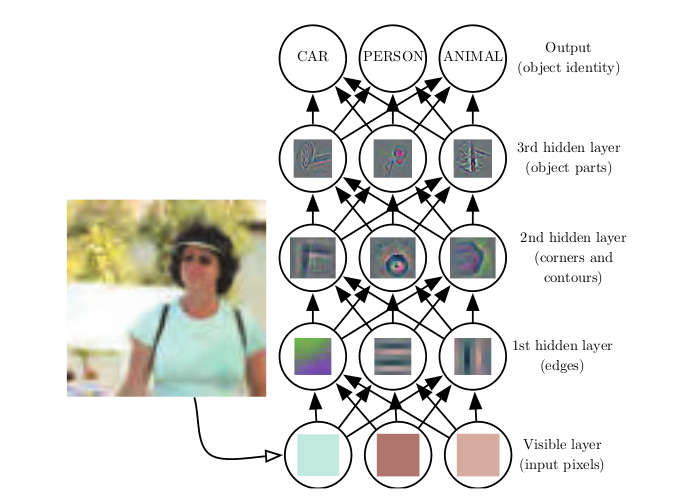
\includegraphics[scale=0.5]{figures/image-classification.png}
    \caption{Image Classification Deep Neural Network @@@IAN}
    \label{fig:dnn_classify}
\end{figure}

\section{Convolutional Neural Networks}

Convolutional Neural Networks (CNN's, sometimes called Convnets), introduced by LeCun in 1989 are a specific and modern neural network architecture. This architecture specializes in working with data which has spatial or grid-like relationships. Some examples include images (e.g. two dimensional grids for grayscale image data), time-series data (which can be seen as a one dimensional grid), or other sequence data. Convolutional neural network have found their way into many successful implementations and are as of today one of the most common (and modern) type of deep neural networks. The name convolutional neural network comes from the mathematical operation of convolution, and it implies that a neural network uses this operation for some operations (feature extraction). To define formally: "Convolutional networks are simply neural networks that use convolution in place of general matrix multiplication in at least one of their layers." @@@IAN Besides convolutions, some other operations are usually required for a successful CNN implementation, like for example pooling, which will be explained later. Convolutional neural networks take inspiration from the animal world. Specifically, some animals have developed parts visual cortexes where information is processed in way that the surrounding information is also taken into consideration. In the case of image processing, for example, this simply means that we no longer look at the image pixel-by-pixel but rather we look at groups of neighbouring pixels. This is a powerful concept in learning and generalization in modern neural networks.

\subsection{Convolutional Kernels}

Convolutional Neural Networks can have many convolutional kernels or convolutional filters. These kernels are used for calculating the convolutions and in them the weights (knowledge) is stored similar to the weights on the synapses of fully-connected neural networks. Here, we explain briefly what are convolutional filters, what is the operation of convolution and what is the motivation behind using convolutions in neural networks.

In the most general mathematical terms, convolution is an operation on two functions of a real-valued argument. In deep learning the term convolution is used when we want to specify that we are using a convolutional operation to process the input data or some hidden layer data. The correct terminology for two parameters to the convolutional operation are: the input and the kernel (or filter). The output of the operation is often called a feature map (map which shows where are some features detected). The data processed in the case of CNN is always a multi-dimensional array (tensor of usually three dimensions: width, height and depth -- for a color image input depth is the color channels) which is used as an input parameter to a convolutional operation and another tensor called kernel. 

The easiest way to explain the convolutional operation in CNN's is by a simple example. In image processing operation of convolution means that a smaller sized image (kernel) is slid over the larger input image. The operation computed during the sliding is a simple element-wise multiplication. If a feature image matches a part of the input image the output of the operation will be a non-zero number in the resulting image (feature map). It is important to say that we do not define convolutional filters, they are learned through back-propagation like other learnable parameters in neural networks. One example of convolutional processing can be seen in Figure \ref{fig:conv}.

\begin{figure}
    \centering
    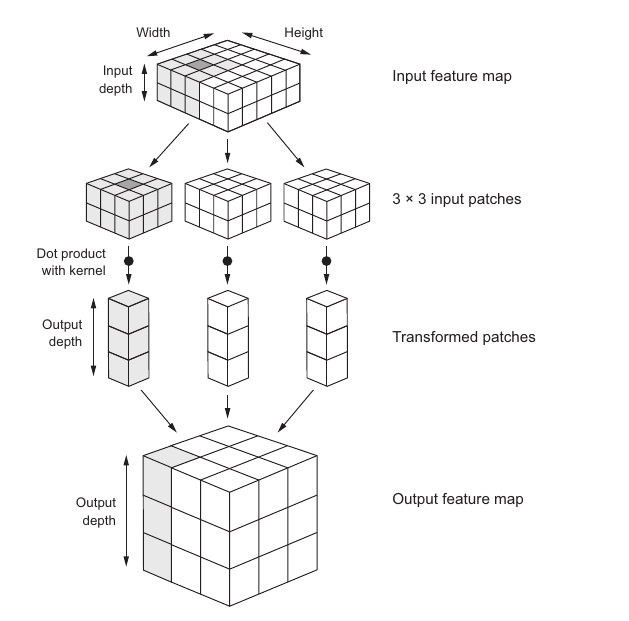
\includegraphics[scale=0.5]{figures/conv-chollet.png}
    \caption{@@@CHO Example of a convolutional operation on input data}
    \label{fig:conv}
\end{figure}

@@@CHO
The main difference between a densely connected layer and a sparsely connected convolutional layer is that the dense layer learns global patterns in input data (e.g. pixel data in an image) and the convolutional layer learns local patterns (e.g. patterns found in images -- edges, shapes etc.).

This approach gives CNN's two interesting properties: patterns they detect are translation invariant (it does not matter where they are in the input data) and they can learn spatial hierarchies of patterns (first conv. layers learns local patterns, the next one learns larger patterns etc. like we described in the previous section).

Convolutional layers in neural networks have two key parameters: size of patches extracted from the input (usually squares of small dimension: e.g. 3x3 or 5x5) and the depth of the output feature map (defined by the number of convolutional kernels). Other than these parameters, we can also define padding (adding data around the input data for compatibility reasons) and stride. Stride defines how a convolutional filter is moved through the input data -- how large is the movement step. 

Another important parameter is downsampling or pooling. We use pooling (usually max-pooling) to reduce the size of the output convolutional feature map. These feature maps are propagated through many convolutional layers and it can be computationally expensive to process them in full. That is why we opt for the down sizing them by using the max pooling operation which only keeps maximum values from parts of the feature map output. Another benefit of this operation is better generalization -- e.g. to classify an object it is not important where it is in the image, but whether it is present anywhere on the image.

@@@ add references below

Convolutional Neural Networks can be and are used for many other image-related and other tasks. Apart from the textbook example of image classification they can be used for image segmentation, object detection, object detection in videos, video classification, image superresolution, sentence classification and many other tasks.

\subsection{ImageNet}

ImageNet Large Scale Visual Recognition Challenge (ILSVRC) is a widely known competition in object detection. A dataset of billions of images and 1000 classes is provided and different research teams compete every year to improve upon state-of-the-art results. ImageNet challenge became widely known around 2020 when Krizhevski et al. demonstrated that CNN's can be used successfully for this use case. The initial CNN model they demonstrated may be simple in today's terms, but it brought down the state-of-the-art error rate of 26.1 percent to a new record of 15.3 percent -- a huge leap forwards. Since then ImageNet challenge is dominated by neural network models, and today's state-of-the-art models have top-5 errors rate as down as 3.6 percent.

Another important consequence of the ImageNet challenge and the reason we mention it here is that it introduced researchers to parameter sharing and transfer learning. For the model to be validated it had to be shared, meaning that it's parameters were publicly available. Most importantly, convolutional kernels were shared and they could be freely used for other tasks. It is quite common today to use pre-trained (meaning frozen, constant) convolutional layers in an image-related neural network. As the ImageNet models are trained from all publicly available images on the Internet, the convolutional layers are incredibly valuable as they contain almost every imaginable image feature there is. In one of our negative models, transfer learning is used as an important step in the training process. 

\section{Recurrent Neural Networks}

Recurrent neural networks (RNNs) introduced by Rumelhart et al. in the 1980s are a type of neural network used for processing sequential data. As convolutional networks are specialized for processing of grid-like inputs, such as images, a recurrent neural network model is specialized for processing sequences of values. As Convolutional Neural Networks can readily work with large images by looking only at their parts, RNNs can usually work with long (or infinite) sequences. Where feed-forward fully connected networks would fail with large sequences limited by their architecture, these specialized models are made to look at parts of sequences in order making them fully scalable. Also, like some CNNs can process images of variable size, RNNs can be made so they can process sequences of variable length.

Jumping from classic fully connected networks to recurrent models requires a special paradigm: parameter sharing across different parts of the model. Parameter sharing makes it possible to apply the neural network model to examples of variable form (different length) and generalize across them. If we are to have separate parameters for each value in time, we could not generalize to sequence lengths not seen during training. Sharing is important also to remove positional correlations in the data. Sentences "I lived in Coimbra in 2020." and "In 2020, I lived in Coimbra" have the same meaning, even though through the eyes of an algorithm they are completely different. Similarly how CNN models are invariant to feature positions in images, we want our sequence models to be invariant to term positions in them. Some 1-D CNN models can be used for sequence models but in comparison to RNNs they are shallow -- they can only look at neighbouring parts of the sequence, without memory.

In practice recurrent neural networks are implemented so they accept in addition to the input a hidden state input which is usually the output of the last time step.

Recurrent can be split into many different categories, to name a few common ones:

1. Recurrent neural networks producing output at every time step, and have recurrent connections between hidden units
2. Recurrent neural networks producing output at every time step, and have recurrent connections only from output of a step to the input to the next step (like in the example above)
3. Recurrent neural networks with recurrent connections between hidden units that accept the entire sequence and then produce a single output value

\subsection{Modern RNNs, memory and attentive models}

In this section we will discuss some of most important sequence models.

One important RNN model to mention is the Sequence-To-Sequence model (seq2seq). This model uses an encoder-decoder architecture to map one sequence to another. The sequences do not have to have same length. This model is used very successfully for Neural Translation Tasks.

One issue that recurrent neural networks have due to the vanishing gradient phenomena (@@@REF) it is very difficult for them to take into consideration states from many time steps before. Two successful approaches to this problems are the gated reccurent unit (GRU) model and the long short-term memory (LSTM) model. Both of these architectures use gates or self-loops to produce paths where gradients can flow for a long period of time. LSTM model especially has found great success in tasks like unconstrained handwriting recognition, speech recognition, handwriting generation, machine translation, image captioning and parsing. @@@ REF od IAN

Neural networks are very good at learning implicit connection in the data, but they lack in the simple task of memorizing of facts. This is due to SGD (stochastic gradient descent) requirement of many presentation of some input before it can be stored in a way in the network parameters. Even stored, the input will not be kept with high precision. Human beings are known to memorize facts though a "working memory" system (Graves et al. 2014). The need for a model that can process information as a sequence of steps (recurrent models) was clear and in 2014 Weston et al. introduced memory networks that include a set of memory cells. Memory networks, at first, required supervised signal to know how to use their memory cells, but in 2014 Graves et al introduced Neural Turing machines which were able to learn whether to write or read data from memory cells without supervision. This allowed self-contained end-to-end memory training with the use of content-based soft attention mechanism. This attention mechanism has become standard way of introducing memory to recurrent neural network models.

\section{Generative Models}

@@@CHO

Even though artificial intelligence and specifically machine learning is mostly used on existing data to find hidden patterns and meaning, it was always known that with some modification, machine learning algorithms can be used to produce new, unseen data. Deep neural networks have been used for many generative tasks such as text generation, image style transfer, image generation etc.

Our languages and artworks all have hidden statistical structures. Learning these structures is what deep-learning algorithms excel at. These models can learn the statistical latent space of images, music, and stories so they can sample this space and create new works with many of the existing characteristics found in training data.

For text generation, recurrent neural networks which are used for sequence modeling as we already mentioned, can be used not only to predict or classify text but rather to write it. Working with generative RNNs can be generalized to any sequence data, not just text. LSTM networks have been used with great success to generate music, for example (e.g. Magenta @@@REF). The process of generating new sequence data is quite straightforward. First, we train a RNN model which is used to predict next items in a sequence e.g. next letter in a sentence. Then, with the model trained we give it some initial starting text (often called conditioning data) and ask it to generate the next value. Then we add that value to the starting text, and repeat the process many times. The loop allows us to create sequences of unlimited length. In sentence modeling, RNN models learn from human written sentences and are able to produce very coherent and meaningful sentences. It is very important to mention sampling strategy. It is not a good idea to use greedy sampling as in normal RNN prediction models. Greedy sampling is a sampling strategy where in every time step the best result is taken. If we were to use such strategy with generative models, we would get repetitive and meaningless sequences. If we introduce stochasticity or randomness to the process, we usually get much better results.

Another area where generative models excel is image processing. DeepDream is an artistic image-modification experiment developed at Google. It quickly became an Internet sensation because it generated some very weird-looking images given an image output. The weirdness came from various artifacts taken from convolutional layers of a CNN trained on the ImageNet dataset. It used reverse convolutions, and gradient ascent on the input image in order to maximize the activation of a specific filter (or many filters, entire layers even) in upper layers of the CNN.

\begin{figure}
    \centering
    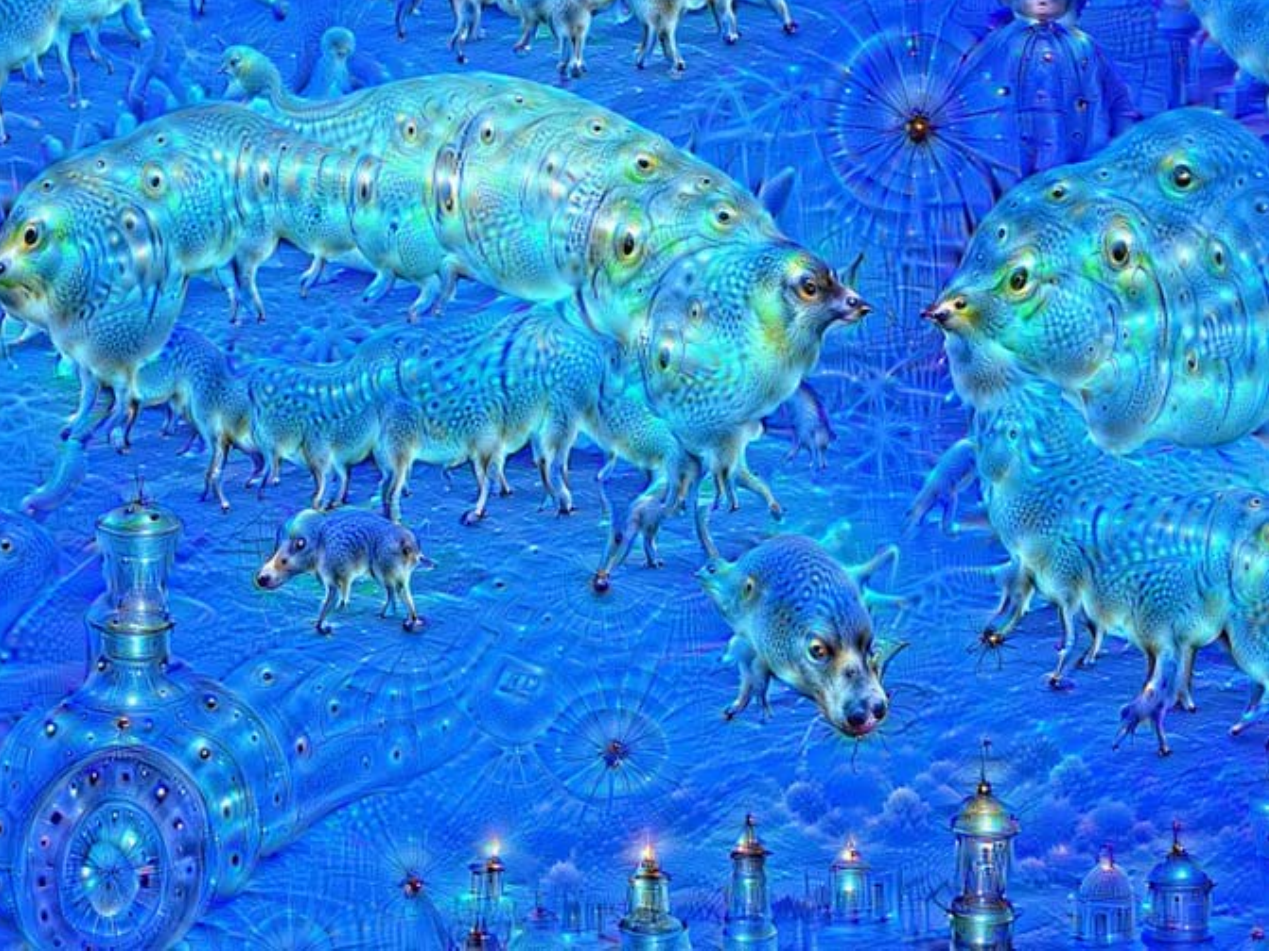
\includegraphics[scale=0.2]{figures/deepdream.png}
    \caption{@@@CHO Example of a DeepDream network output image}
    \label{fig:deepdream}
\end{figure}

Another image processing generative network which received major praise was the Neural style transfer algorithm. This algorithm can be used to transfer artistic style from one image to another while preserving content. Style, in this context means textures, colors and visual patterns found in images, while content represents the structure of an image. The style transfer is achieved by implementing a specific loss function and minimizing it, like in almost all neural network applications.

The loss function would look something like this:

\begin{multline*}
loss = distance(style(reference_image) - style(generated_image))\\
+ distance(content(original_image) - content(generated_image))
\end{multline*}

In this formula distance function is a norm function such as the L2 norm, content is a function that takes an image and computes a content representation, style is a function which does the same for style. Minimizing this function causes both the style and content values of two images to be closely related. The interesting part of this algorithm of course is how to define the content and style loss functions. To put it simply we can use convolutional layers at various depth to extract image representations. The depth is very important because we know that earlier convolutional layers contain low-level local information about an image, and the deeper layers contain more abstract global information. The style loss has a bit more additional complexity: style can be captured at all layers in the network, and that is why Gatys et al. (the original Neural Style Transfer authors) suggest usage of Gram matrices which are the inner product of feature maps in a convolutional layer. This inner product can be understood as a map of correlations between layer's features.  These feature correlations contain the statistics of the patterns of a particular spatial scale, which empirically were found to be the textures in an image.

\begin{figure}
    \centering
    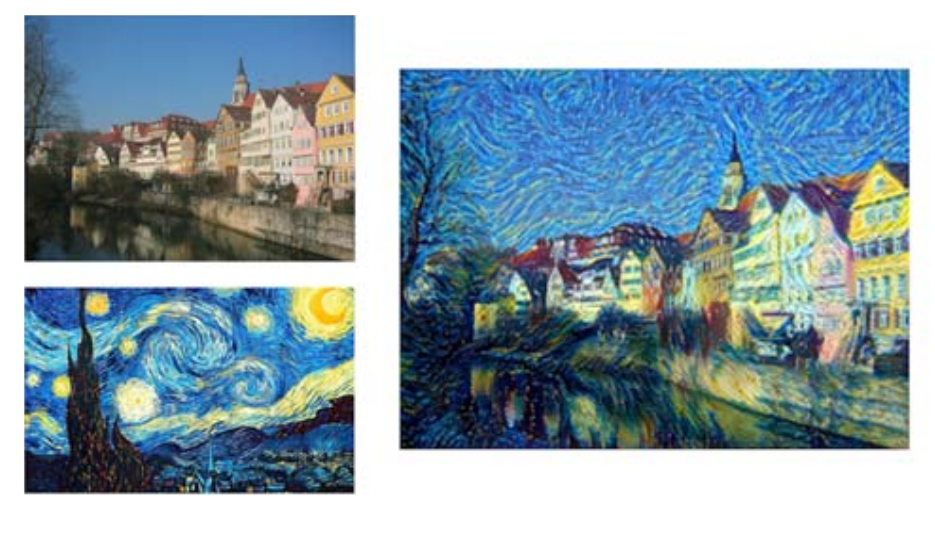
\includegraphics[scale=0.45]{figures/nst.png}
    \caption{@@@CHO Example of a Neural Style Transfer application. On the top left we have an input image -- a photograph. On the bottom left we have Van Gogh's Starry Night, used to extract style. And on the right we have the resulting image, content from the input image, style from the Starry Night.}
    \label{fig:nst}
\end{figure}

Another popular generative method is the Variational Autoencoder (VAE) model. Autoencoders are a special type of neural networks where the input and the output are identical. The benefit of these models comes from their architecture. All autoencoders have such structures that the input is reduced in size until one point in the network and then increased in the next. These two parts of the model are called the encoder and the decoder and the middle point in the network is called the bottleneck. When a model like this is trained it is forced to learn a compressed representation of the input so it can use that representation to decompress it and produce that input again as the output. Autoencoders can also be used for clustering, anomaly detection and many other unsupervised tasks -- in which traditionally neural networks are not used. 

Autoencoders are also generative models. If we take the decoder part and feed it some random inputs, we will get an output of some sorts which would be similar to some parts of our training dataset. This way of sampling from latent space of images for example to create new images or modify existing images is one of the most popular and successful applications of generative models today. We mentioned latent space and we define it as a low-dimensional vector space where any point can be mapped to a realistic-looking image. When we create this latent space we can sample from it, deliberately or at random and the output becomes a previously unseen input (image). VAEs learn latent spaces that are well structured where specific directions in the multidimensional vector space encode meaningful variations in data. If we train a VAE with a dataset of portraits for example, one such direct would be hair color or whether the person in the image is smiling. At the end we need to emphasize differences between traditional autoencoder models and the variational autoencoder model mentioned here. VAEs differ from normal AEs in that we impose various constrains on the latent space definition so we force the model to learn better representations of features found in input data. For example we can limit the latent space to be low-dimensional and sparse, forcing the model to learn better. When comparing latent spaces of normal AEs and VAEs it is apparent that VAEs have better defined structure. This is because VAEs in addition to compressing input data into a fixed point in the latent space also turns the data into parameters of a statistical distribution (mean and variance). This means we assume that the input data has been generated by a statistical process and that the randomness of the process should be considered during encoding and decoding. The mean and variance parameters are then used to randomly sample one element of the distribution to decode that element to the input to the model. The randomness of this process improves both the latent space structure and continuity and the robustness of the whole process.

\subsection{Adversarial Learning}

Generative Adversarial Networks (GANs) which were introduced in 2014 (Goodfellow et al) are another generative neural network model. They also can learn latent spaces of images (or other data) similar to VAEs. GANs can generate fairly realistic synthetic images by forcing them to be statistically indistinguishable from the real images.

Easiest way to explain generative adversarial networks is to imagine someone trying to forge a Picasso painting. In the beginning the forger will perform poorly because lacks authenticity. However the forger will then mix his own work with actual Picasso paintings and show them to a trained art dealer. The art dealer will tell him what he thinks about the pictures and how he was able to distinguish the real pictures from the fake ones. He will also provide information about what he looks for in authentic Picasso pictures. As this process is repeated, the forger will use this information to become better and better at forging the pictures until the art dealer cannot distinguish between actual Picasso paintings and the forger created ones.

This is exactly how a GAN works. It is joint model of two networks: a forger (generator) network and an adversary network. Hence the name generative adversarial networks.

The generator network takes a random vector (random point in the latent space) and produces a synthetic image. The adversary network takes as input image and predicts whether the image is from the training set or from the generator network. The generator network is trained to fool the adversary network, as it evolves and creates more and more realistic looking images. The adversary (sometimes called discriminator networks) meanwhile judges the work of the generator network.

GANs and other adversarial learning methods have found their use not only for generating data but also for testing the robustness of trained neural networks. They can be used for input modification (such as perturbations or occlusions) which are then use to trick the trained network into a wrong classification output. Usually, the goal is not just to modify the inputs so it wrongly classified but also for that input to remain recognizable to the human eye. The modified input image can look entirely normal but to be wrongly classified by a performant model. This is called an adversarial attack and we will focus on this topic later in this manuscript.

\subsection{Deep Reinforcement Learning}

Another great success in the field of Machine Learning and specifically Deep Learning was the introduction of deep reinforcement learning algorithms. In the scene set, an agent enabled with a powerful neural network model must learn to perform some task by trial and error, with any guidance from its human operator. DeepMind demonstrated that this type of learning algorithm can be taught to play old Atari games, reaching and surpassing human levels of play. Deep Reinforcement Learning models also made headlines when AlphaGo, a trained agent playing the board game Go, was developed and defeated world champions on several occasions. Another area where these algorithms have found great success is in robotics and also in self-driving cars -- a very popular field nowadays. We will cover deep reinforcement learning in more detail later in this manuscript.

\section{Future of Deep Learning and Towards Artificial General Intelligence}

This section contains some authors speculations about the future of Deep Learning and its uses.

Moving forwards towards new chapters in the field of Artificial Intelligence we can expect that Deep Learning will move away from model only performing pattern recognition and can achieve limited local generalization. We will need to develop model able to develop abstractions and reasoning while achieving extreme global generalization. Current AI programs that are able to reason are mostly hardcoded by their programmers, even in most advanced Deep Reinforcement Learning approaches. In DeepMind's AlphaGo, for example, most of the learned intelligent behaviour is designed and coded by expert programmers (e.g. Monte Carlo Tree Search) and learning from data only happens in part of the system (value and policy networks). In the future AI systems should be able to "code themselves" without human involvement. 

The current neural network models are limited by their programming to be a set of geometrical operations on an input vector. A model able to freely modify its own code with a set of defined programming language rules would be able to achieve much better results in all scenarios. In a way, computer programs could be replaced with machine learning models which are self-programmed. One interesting research field related to this is neural program synthesis. Program synthesis consists of automatic generation of simple programs by employing search algorithms (even genetic, as in genetic programming) to explore a large space which contains all possible programs. The search stops when a program with a matching specification is found. The specification is often given as a pair of input-output pairs which is of course reminiscent of machine learning. The difference is that instead of learning parameter values (weights) in a hardcoded neural network we generate new source code in a discrete search process. 

These new programs won't be differential like the hardcoded neural network models of today. Therefore backpropagation will need to be replaced with a more suitable method. Whether that is genetic algorithms, evolution strategies, alternating direction of multipliers (ADMM) or other method, some things will need to change. Gradient descent will probably stay because the gradient information will always be useful for optimizing differentiable parametric functions.

Of course, all Deep Learning models will eventually become portable, in a way that they can be trained and ran or various mobile hardware. We are already witnesses of mobile chip development specifically with neural network image processing in mind. Many of the mainstream machine learning frameworks and libraries already support running models on mobile phones and other portable computers. Different concepts like network compression, pruning and quantization exist today to ease the transition of resource-intensive models to relatively weak but increasingly stronger devices we carry today.

In short, this perpetually learning model-growing paradigm can be interpreted as AGI (artificial general intelligence) where models can learn and learn what to learn and how to learn. This is not something easily achievable and with no clear way of doing it, it will be years before we are close. When done, however, our lives will change significantly.

\section{Modern Neural Network Concepts}

In this section, we briefly go over some of the state-of-the-art concepts and research taking place in the field of Deep Learning.

\subsection{AutoML}

Automatic machine learning or AutoML is a fairly new concept in the field of Machine Learning. Today, most of the machine learning architectures are still defined by their human operators. In the future, and today already we have some methods of unsupervised architecture optimization. This allows the model to adjust not only its parameters but its architecture as well. Some problems, it has been shown, can be solved better and easier with a specific architecture which is hard to conjure. 

Going further, the main job of a deep learning expert nowadays is to structure the training data and come up with a good set of hyperparameters and a good architecture for a specific problem. Needless to say, this is a lot of work. With AI's help several steps of this process can be automated. The data preparation (or data cleaning, as it is often called) is very difficult to automate, because it often requires domain knowledge as well as a clear, high-level understanding of what is to be achieved and in what way. Hyperparameter tuning, however, is a different story. It can be seen as a simple search procedure, or a trial-and-error process. In this case, we already know the ideal outcome which is the minimization of the loss function in training. But we want to find the best hyperparameter values. It is possible today to use an AutoML framework, and set it up to find best hyperparameter values for a certain problem. The most basic AutoML implementations would define arrays of possible hyperparameter values and try various combinations of them. The parameters can be basic values such as learning rate or momentum but they can also be more complex like for example number of layers or number of units in a hidden layer etc. One good example of this method is NAS or Neural Architecture Search method.

\subsection{Transformers}

Transformers are a deep learning model introduced in 2017. @@REF They are used specifically for sequential data similarly to recurrent neural networks. Unlike recurrent neural networks Transformers do not need to process the input data in order making them easier to parallelize with loss in model quality when compared to state of the art RNN models like LSTMs for example. This means that larger and more complex models are possible to train and use, and also that larger amounts of data can be used for training. One such use case is of course in text processing where Transformers are currently state of the art models used for various tasks like machine translation, document summarization, document generation, named entity recognition, and others. They can also be used for other sequential data like for example biological sequences. One research group even showed that a specialized transformer architecture can be used for playing chess. In 2020, many language models were made available by leaders in the Natural Language Processing field. Most notable include: GPT-3, GPT-2, BERT, XLNet, RoBERTa and others. These models attracted lot of attention because of their ability to generate stories or volume of texts almost indistinguishable from human written text. 

Speaking of attention, it is important to mention it here. In the paper "Attention is all you need" where Polosukhin et al. introduce Transformers it is shown that attention is a very important parameter in neural network models used for sequential data. As we briefly mentioned in previous sections regarding recurrent models, today's gated recurrent models (LSTM, GRU, etc.) use gates to simulate memory. Attention mechanism not only allows the RNNs to remember many previous states (solving the problem with older RNN models) but to distinguish what previous states or previous information is important. In a neural machine translation task, for example, it is obviously important to look at entire sentences for translation instead of just the previous time step. The authors of the mentioned paper use attention-like method but without the requirement for sequential processing of data, allowing parallelization. Lastly, transformers are still an encoder-decoder architecture similar to other models we mentioned in this manuscript.

% https://en.wikipedia.org/wiki/Transformer_(machine_learning_model)

\subsection{Federated Learning}

As mobile devices and sensory IoT devices become more and more involved in machine learning workloads the need for decentralized training or collaborative learning is increasingly apparent. Federated learning is a machine learning technique that trains a model across multiple devices. These devices can vary in architecture, power or other capabilities. One specific point is that in federated learning there is no single centralized data store where the training data resides. It is rather split into chunks and every device (node) has limited amount of information for training. In other words, nodes rely on each other for a performant model. This is very useful in scenarios where many devices gather data (e.g. sensors in factories), because that data can be processed immediately. Another benefit is from the data sharing standpoint, as the data does not necessarily need to be shared across various devices addressing critical issues such as data privacy, data security, data access rights and access to heterogeneous data.

There are many ways in which federated learning can be implemented. One closest to other topics in this manuscript is of course the decentralized deep neural network model. In this scenario local models are created and trained with local data samples and parameters such as weights and biases of the model are then shared with other nodes. Other nodes choose how to use the knowledge shared with them, usually this knowledge (parameters) is averaged with local parameters and then taken into consideration. Federated stochastic gradient descent (FedSGD) and its generalization Federated averaging (FedAvg) are commonly used.

It is important to mention that federated learning is not the same term as distributed learning. Distributed learning has a different purpose: to train a single model across many devices. The single model is often too large for a single node or the training time is too long because of a large dataset. That is why we can use a set of computing nodes which are used for their processing power.

Federated learning technique is used a lot for online learning (additional training for existing models) as well as for critical systems where privacy is a priority. Some examples include self-driving cards, Industry 4.0 use-cases (smart manufacturing processes), medicine and others. Federated learning is also accelerated by recent hardware developments both in ARM chips and in network infrastructure like 5G broadband networking.

\part{Negative Learning}

In this part of the manuscript we define negative learning as a term taken from cognitive psychology and we describe ways of introducing it to the field of Deep Learning.

\section{Introduction to Negative Learning}

Negative learning in psychology can be defined in many ways. One way to define it is learning with a negative reward or a penalty. This approach can be directly applied to agent-based algorithms like for example, Reinforcement Learning algorithms. Learning with a negative reward or penalty is described so that an agent can be penalized for its actions if they are deemed inadequate. For a self-driving car for example some actions can be seen as positive and some can be seen as negative. Positive action would be for example stopping at the stop sign, while a negative action can be crashing or speeding. When training these agents, it is necessary to do so with both positive and negative examples of behaviour. This approach takes inspiration directly from human behaviour. Children for example are often disciplined when behaving in a inappropriate way.

An algorithm which only uses negative samples for learning, hoping that if it knows all the actions which should not be taken, will be able to deduce the correct (positive) action, would be called a negative learning algorithm. It is difficult to say whether it is a good approach for an algorithm to only learn using negative samples. We will see in later sections that this is possible.

Negative learning can be defined also in the realm of two large sub groups of machine learning problems: classification and regression.

In classification tasks a machine learning algorithm is needed to classify certain input data. We differentiate binary (two-class) and multi-class classification. The algorithm outputs to which class from a predefined set of classes the input belongs to. It does so based on its features. During training many examples of the input and output data are presented to the algorithm. It learns and changes its parameters so it can classify all the provided input-output examples. Negative learning in this case can be defined in several ways. We could ask for example to what classes the input date does not belong. Another example would be if we asked what features need to exist so we know the input data does not belong to a certain class. We will visit these questions (and implement them) in the following parts of this manuscript.

Similarly, in a regression task a machine learning model is tasked to output a real numbered value for a certain set of inputs. A negative learning model in this case would be able to tell us not what the expected output for a certain point is, but rather what scope of output values is not expected. We could also model regression tasks as classification tasks, if we were to discretize the data of course.

There are other ways to define negative learning, but in this manuscript we will focus on the three mentioned problems here: problem of classification, regression and agent-based environments.

\section{Reasoning and possible benefits of Negative Learning techniques}

There are many reasons why one would need to use techniques we describe here. 

For one, positive examples may be unavailable during training. If we have only negative examples for the model to learn from we need a model capable of understanding that it is dealing with negative information.

Another reason is for increased robustness. As we will discover later, negative models in some scenarios are proven to be more robust than their positive counterparts. Robustness here means that the model will have same or increased accuracy in difficult situations. These difficult situations can be defined as situations where traditionally machine learning models have issues: missing data, partial data, adversary attacks etc. Negative samples can be seen as additional information available for our model. This additional information can be very useful in difficult scenarios when a model is not certain. 

One more reason is increased performance of the models. Similarly to robustness if the models use this additional negative data in a correct way, they can converge quicker or have increased accuracy, precision or other important metrics.

We will mention more use cases specifically for Negative Deep Learning in the next chapter.

\section{Policy-based algorithms and Negative Learning}

Policy-based algorithms are a natural contender for negative learning. As mentioned earlier, policy-based algorithms (e.g. reinforcement learning algorithms) learn a policy function based on which an agent behaves in an environment. This policy function is learned in an iterative process of trial and error where the agent tests various actions that are possible and how they affect the environment. This policy function depends largely on the reward/penalty function where the agent is given a numeric value denoting a positive (reward) or a negative (penalty) outcome of the last action performed.

Negative learning in the case of policy-based algorithms can be seen as using only negative values for the reward/penalty function. The policy learned in this way would only have negative knowledge in its definition. In other words, the agent would only know what not to do in certain situations. The action chosen would be a randomly selected one, but the chosen action would certainly not be an action which the policy function knows to incur a penalty. This is one of the purest forms of negative learning, where the agent only knows what actions are not to be taken.

\section{Negative Learning in other algorithms}

In the task of binary classification, literature often separates the date into two categories: positive and negative data. Positive meaning the data which has a "True" value and negative meaning data with a "False" value. It is easy to define negative learning as learning from only the negative parts of the data. One has to be careful in these scenarios as overfitting is highly probable for various models. Overfitting is a case in machine learning when a model highly favours one output class in a classification task. If we are only to train with negative data, it is highly likely that our algorithm would learn to always output negative outcomes even when data for a positive outcome is given. Negative Deep Learning as we will see later makes more sense for multi-class classification problems but can also be used in certain ways for binary classification.

One more interesting contender for negative learning is in the problem of anomaly detection. In anomaly detection tasks, an algorithm is trained so it can recognize certain irregularities in data. These irregularities are called anomalies and can be defined as anything which differs from the normal data that the model saw during training. However we can also define these models in reverse. 

In anomaly detection problems algorithms (such as autoencoders) are trained on filtered data which does not have anomalies. In a way the model is forced to learn and memorize normal data so that later on it can recognize when anomalous data is given. Negative learning version of this algorithm would be to train the model on only the negative data (or anomalies). That way an algorithm would learn how anomalies look like and would learn to recognize them among normal data points. Some literature defines this as a traditional positive learning approach, so it is very interesting that traditional anomaly detection can be seen as a negative learning method.

\chapter{Negative Deep Learning}

In this chapter we begin to define negative deep learning methods and provide an overview of possible implementations and use cases. We also provide several necessary definitions before we move to concrete examples in following chapters.

\section{Negative Deep Learning -- Introduction}
\section{Possible Models of Negative Deep Learning}
\subsection{Missing Features}
\subsection{Partial Input Sample Training}
\subsection{Negative Output Learning}
\subsection{Ensemble Networks and upgrades of existing models}
\subsection{Agent Environments}
\section{Negative Deep Learning Use Cases}
\subsection{Object Detection and Image Classification with Occlusions}
\subsection{Neural Network Robustness}
\subsection{Neural Adversarial Attacks}
\subsection{Black-box attacks}
\subsection{White-box attacks}
\subsection{Negative Neural Networks for Regression Tasks}
\subsection{Other uses}

\part{Classification Based On Missing Features}

\chapter{Introduction}
\section{Intuition behind Missing Feature Representations}
\section{Examples of deduction with Missing Features Classification}

\chapter{Motivation}
\section{Robustness of Image Classifiers}
\section{Partial Input Classification}

\chapter{Implementation}

\section{The Negative Function}
\subsection{Activation Function Experiments}
\subsection{Negative Convolutional Kernel Experiments}
\subsection{Influence of the Negative Function in forward and backward passes}
\subsection{Influence of multiple-step training}
\subsection{Negative feature selection process}
\subsubsection{Detecting relevant features per-class for negation}

\section{Training process}

In this section training processes related to the negative learning method are described with the focus on two very important processes: multiple phase training and convolutional kernel freezing. To successfully implement the classification based on missing features model our experiments have shown that both of these techniques have to be used.

\subsection{Multi-phase training}

During the Negative Deep Learning model/hypothesis testing one interesting concept was used -- multi-phase training. Multiple phase training is a training process where after a number of training epochs some layers are frozen and reused and some of the layers are reset. In a way, multiple phase training is a regularization technique similar to Dropout with P=1.0 where some layers are completely destroyed and retrained during training. 

In our concrete example multiple phase training was used to extract and reuse convolutional layers from an image classification model. After a number of epochs all the convolutional kernels were extracted and used in other (negative) models.

\subsection{Convolutional Kernel Freezing}

For most of here mentioned models we use freezing of convolutional kernels. Freezing is a process of setting convolutional layers as fixed, constant values after they have been learned. The freezing of the convolutional layers is important from the analysis standpoint as we want to test our model modifications which are currently after the convolutional blocks. If we were not to freeze the convolutional layers, they would change their parameters during training -- and this is not desired behaviour. 

Freezing of the layers is a procedural process where one has to iterate through convolutional filter parameters (conv. kernels) and mark them as constant. In the PyTorch framework this is done with the "required\_grad" field.

Freezing of the convolutional layers (or other parts of a neural network models) is a common technique when using pre-trained models. The idea behind pre-trained models is simple: a model trained on a dataset (usually large, not easy to retrain) is extended with few layers on top to be used for some different task. One example where this approach is popular is with image classification. There, it is common to use very deep and complex models trained on the ImageNet Dataset as frozen feature extractors. In addition, a simple fully-connected neural network is added "on-top" of the ImageNet model and trained to classify custom image datasets.

\chapter{Testing}

\section{Results on the MNIST and PMNIST datasets}
\subsection{PMNIST dataset}
\subsection{Corner occlusions}
\subsection{Image Perturbation Experiments}
\subsection{Differences in activation functions}
\section{Robustness to Adversarial Attacks}

\part{Synergy of Traditional and Classification Based On Missing Features}

\chapter{Overview of Ensemble Learning Techniques}
\section{Experiments with different network joining techniques}
\subsection{Addition}
\subsection{Multiplication}
\subsection{Fully-connected blocks}

\chapter{Experimental hypothesis}
\section{The need for ensemble "synergy" models}
\section{Observing probabilities of normal and negative models}

\chapter{Implementation}

\section{Classic Synergy}
\section{Trained Synergy}
\section{Influence of multiple-phase training in synergy networks}

\chapter{Testing and Results}

\section{Model definitions}
\section{Performance of normal and negative models}
\section{Synergy Performance}
\subsection{Select Case-by-case analysis of the Synergy network}
\section{Occlusion Experiments}
\section{Softmax benefits regarding both networks}
\section{Robustness to Adversarial Attacks}

\part{True Negative Deep Learning}
\chapter{Introduction}
\section{Goals and Motivation}
\section{Problem definition}

\section{Defining "True" Negative Deep Learning models}

\chapter{Siamese Neural Networks}
\section{Triplet Loss Function and our modifications}
\section{Initial experiments and results}

\chapter{Noise Contrastive Estimation Models}
\section{Negative sampling}
\section{NCE models for Natural Language Processing}

\chapter{Other models}

\part{Negative Deep Learning in Agent Environments}

\chapter{A short introduction to Deep Reinforcement Learning}
\section{Deep Q Learning}
\section{Other models}

\section{Motivation and use-cases}
\section{Negative Rewards and Punishments}
\section{Overview of existing models}

\chapter{Testing environments}
\section{OpenAI Gym Environments}
\section{Infinite Negative Testing Environment}
\subsection{Collision Avoidance in Open Environments with Negative Deep Reinforcement Learning}

\chapter{Results}
\section{Convergence time comparison}
\section{Model performance}

\part{Appendices}
\chapter{Experiment Reproducibilty and Determinism}
\chapter{Source code}
\chapter{Open Source Licences}
\backmatter

% there is no index, so it's disabled
% \printindex

% \skica{} use raggedright, had problems with urls and dois not breaking proper
% maybe there are better solutions
{
  \raggedright
\printbibliography[heading=bibintoc]
}

% --------------------------------

\chapter{Prošireni izvod}



% --------------------------------

\chapter{Short Biography}


Nemanja \cite{novak2010comparison}

\vfill


\begin{tabbing}
  \hspace{0.7\textwidth} \= nebitan tekst \kill
  Novi Sad, 2020 \> Nemanja Milošević
\end{tabbing}

\begin{otherlanguage}{serbian}
\chapter{Kratka biografija}

Nemanja

\vfill


\begin{tabbing}
  \hspace{0.7\textwidth} \= nebitan tekst \kill
  Novi Sad, 2020. \> Nemanja Milošević\\
  \\
  \> \makebox[0.3\textwidth]{\dotfill}
\end{tabbing}

\end{otherlanguage}

\newcounter{allpages}
\setcounter{allpages}{\value{frontmatterpage}}

\newcounter{mainpages}
\setcounter{mainpages}{\totalpages}

% offset the last increase
\addtocounter{mainpages}{-1}

\addtocounter{allpages}{\value{mainpages}}

\chapter[Ključna dokumentacijska informacija]{\Large Univerzitet u Novom Sadu\\
          Prirodno-matematički fakultet\\
          Ključna dokumentacijska informacija}
 
\noindent
\begin{tabbing}
  \hspace*{.3\textwidth}                                           \= \hspace*{.7\textwidth}        \kill
  Redni broj:                                                      \>                               \\
  RBR                                                              \>                               \\
  Identifikacioni broj:                                            \>                               \\
  IBR                                                              \>                               \\
  Tip dokumentacije:                                               \> Monografska dokumentacija     \\
  TD                                                               \>                               \\
  Tip zapisa:                                                      \> Tekstualni štampani materijal \\
  TZ                                                               \>                               \\
  Vrsta rada:                                                      \> Doktorska disertacija         \\
  VR                                                               \>                               \\
  Autor:                                                           \> \autor                        \\
  AU                                                               \>                               \\
  Mentor:                                                          \> dr Miloš Racković              \\
  MN                                                               \>                               \\
                                                                   \>                               \\
  Naslov rada:                                                     \> 
    \begin{minipage}[t]{.65\textwidth}
    \naslovsr
  \end{minipage}                                                                                    \\
  NR                                                               \>                               \\
  Jezik publikacije:                                               \> engleski                      \\
  JP                                                               \>                               \\
  Jezik izvoda:                                                    \> srpski/engleski               \\
  JI                                                               \>                               \\
  Zemlja publikovanja:                                             \> Srbija                        \\
  ZP                                                               \>                               \\
  Uže geografsko područje:                                         \> Vojvodina                     \\
  UGP                                                              \>                               \\
  Godina:                                                          \> 2021                          \\
  GO                                                               \>                               \\
                                                                   \>                               \\
  Izdavač:                                                         \> autorski reprint              \\
  IZ                                                               \>                               \\
  Mesto i adresa:                                                  \> Novi Sad, Trg D. Obradovića 4 \\
  MA                                                               \>                               \\
                                                                   \>                               \\
  Fizički opis rada:                                               \> \arabic{numchapter}%
  /\arabic{allpages} (\roman{frontmatterpage} + \arabic{mainpages})%
  /\arabic{citenum}%
  /\totaltables%
  /\totalfigures%
  /0%
  /\arabic{chapter}                                                                                 \\
  \hspace*{2\parindent}
  (broj poglavlja/strana/lit. citata/tabela/slika/grafika/priloga) \>                               \\
  FO                                                               \>                               \\
  Naučna oblast:                                                   \> Računarske nauke              \\
  NO                                                               \>                               \\
  Naučna disciplina:                                               \> Mašinsko učenje
            \\
  ND                                                               \>                               \\
  Predmetna odrednica                                              \>                               \\
  PO                                                               \>                               \\
  Ključne reči:                                                   \> 
    \begin{minipage}[t]{.65\textwidth}
      Veštačka inteligencija, Mašinsko učenje, Duboko učenje,
      Neuronske mreže, Konvolutivne neuronske mreže, Robustnost,
      Robustnost neuronskih mreža, Negativno učenje
    \end{minipage}                                                                                  \\
  UDK                                                              \>                               \\
  Čuva se:                                                         \>                               \\
  ČU                                                               \>                               \\
  Važna napomena:                                                  \>                               \\
  VN                                                               \>                               \\
  Izvod:                   \`
  \begin{minipage}[t]{.8\textwidth}
  U današnje vreme upotreba dubokog učenja radi prepoznavanja određenih paterna u podacima postala je nezamenljiv alat u mnogim sistemima. U kritičnim sistemima pogotovo, duboke neuronske mreže se često koriste čak i u scenarijima koji direktno utiču na naše živote. Upravo to je razlog što se u poslednje vreme u istraživanju sve više stavlja akcenat na duboko razumevanje ovih modela i na modele koji su dokazano pouzdani, robusni i sigurni za upotrebu.

U ovoj doktorskoj disertaciji istražujemo negativne modele dubokog mašinskog učenja kao novi pristup razvoju modela sa visokim performansama i još važnije sa povećanom robustnošću i pouzdanošću u poređenju sa modelima današnjice. Takođe se bavimo nadogradnjama postojećih modela sa našim negativnim pristupom i pokazujemo kako se postojeći modeli mogu unaprediti bez velikih promena u arhitekturi.

Kod modela za klasifikaciju slika (danas najrasprostranjenija primena dubokih konvolutivnih neuronskih mreža) pokazaćemo kako se ovi modeli mogu nadograditi i izmeniti kako bi u obzir uzimali i negativne osobine -- one osobine koje znamo da postoje a nisu trenutno prisutne u ulaznim podacima.

Za sve modele predstavljene u ovoj disertaciji biće prikazana duboka analiza procesa kao što su negacije osobina, negativne aktivacione funkcije, zamrzavanje slojeva neuronskih mreža, transfer znanja iz jedne mreže u drugu, fine-tuning pristup treniranju, inverzije konvolutivnih filtera i drugo.

\end{minipage}\\

\ \`
\begin{minipage}[t]{.8\textwidth}
  Dodatno znanje, u obliku negativnog znanja, može biti veoma bitan faktor u učenju i kreaciji modela koji imaju povećanu preciznost, pouzdanost i robustnost, pogotovo u teškim situacijama. Definišemo teške situacije kao one situacije u kojima je model suočen sa podacima koji su izmenjeni ili teži za razumevanje na neki način, bilo na prirodan način ili veštački način. Na primer, modeli predstavljeni u ovom radu su testirani u slučajevima parcijalnih ulaza i okluzija gde su delovi ulaznih podataka odstranjeni ili zaklonjeni na neki način. Negativni modeli u ovakvim situacijama imaju znatno više performanse u poređenju sa običnim, tradicionalnim modelima iste arhitekture. Za veštački generisane situacije, govorićemo o adversarijalnim mrežama, podacima i napadima i kakve su performanse naših negativnih modela kada se suoče sa takvim podacima. Testirani su black-box i white-box adversarijalni napadi i odabrani su oni napadi koji danas predstavljaju najnaprednije moguće metode za namerna kvarenja modela dubokog učenja.

U ovoj disertaciji takođe uvodimo pojam mreže sinergije, koja predstavlja spoj normalne i negativne mreže i kao takva se može koristiti i primeniti na bilo koji postojeći model. U sinergiji deo mreže ili cela mreža se dodaje na postojeći model u kombinaciji sa određenim modifikacijama kako bi se uključilo negativno duboko učenje. Pokazaćemo da ovakvi modeli imaju još više performanse u poređenju sa negativnim modelima i eksperimentisaćemo sa raznim načinima spajanja mreža. Model sinergije će biti testiran na CIFAR10 skupu podataka dok su negativni modeli razvijani i testirani na MNIST i EMNIST skupovima podataka.

Na kraju, govorićemo o modelima koji koriste "pravo" negativno učenje, a to su oni modeli koji koriste samo negativno znanje za učenje. Biće dat prikaz postojećih sličnih modela kao što su Negative Sampling modeli, Noisy Label Classification modeli i modeli koji koriste Noise Contrastive Estimation. Naš fokus je na dva modela za koje ćemo predložiti i implementirati nadogradnje a to su: negativna Deep Q-Learning agentska neuronska mreža i negativna sijamska Triplet Loss mreža. Oba ova modela mogu biti korišćena uz pomoć samo negativnih podataka, u nekim slučajevima za potpuno treniranje a u nekim slučajevima kao vid regularizacije.
    \end{minipage}                                          \\
  IZ                       \>                               \\
  Datum prihvatanja teme od strane \>                       \\
  Senata:                 \> 25.06.2020.                     \\
  DP                       \>                               \\
  Datum odbrane:           \>                     \\
  DO                       \>                               \\
  Članovi komisije:        \>                               \\
  \hspace*{\parindent}
  (Naučni stepen/ime i prezime/zvanje/fakultet) \>          \\
  KO                       \>                               \\
  Predsednik:              \`
    \begin{minipage}[t]{.7\textwidth}
    dr Srđan Škrbić, redovni profesor,\\
    Univerzitet u Novom Sadu, Prirodno-matematički fakultet
    \end{minipage}                                          \\
  Mentor:                    \`
    \begin{minipage}[t]{.7\textwidth}
    dr Miloš Racković, redovni profesor,\\
    Univerzitet u Novom Sadu, Pri\-ro\-d\-no-ma\-te\-ma\-ti\-č\-ki fakultet
    \end{minipage}                                          \\
  Član:                    \`
    \begin{minipage}[t]{.7\textwidth}
    dr Miloš Radovanović, profesor,\\
    Univerzitet u Novom Sadu, Prirodno-matematički fakultet
    \end{minipage}                                          \\
  Član:                    \`
    \begin{minipage}[t]{.7\textwidth}
    dr Jelena Slivka, docent,\\
    Univerzitet u Beogradu, Fakultet tehničkih nauka
    \end{minipage}                                          \\
  Član:                    \`
    \begin{minipage}[t]{.7\textwidth}
    dr Vladimir Lončar, naučni saradnik,\\
    Institut za fiziku, Zemun
    \end{minipage}                                          \\
\end{tabbing}
%%%%%%%%%%%%%%%%%%%%%%%%%%%%%%%%%%%%%%%%%%%%%%%%%%%%%%%%%%%%%%%%%% 5%%%%%%%%%%%%%

\chapter[Key Words Documentation]{\Large University of Novi Sad\\
          Faculty of Science\\
          Key Words Documentation}
 
\noindent
\begin{tabbing}
  \hspace*{.3\textwidth}   \= \hspace*{.7\textwidth}        \kill
  Accession number:        \>                               \\
  NO                       \>                               \\
  Identification number:   \>                               \\
  INO                      \>                               \\
  Document type:           \> Monograph documentation       \\
  DT                       \>                               \\
  Type of record:          \> Textual printed material      \\
  TR                       \>                               \\
  Contents code:           \> Doctoral dissertation             \\
  CC                       \>                               \\
  Author:                  \> \autor                  \\
  AU                       \>                               \\
  Mentor:                  \> Dr.~Miloš Racković          \\
  MN                       \>                               \\
                           \>                               \\
  Title:                   \>
    \begin{minipage}[t]{.7\textwidth}
      \naslov
    \end{minipage}                                          \\
    TI                       \>                               \\
    Language of text:        \> English                       \\
    LT                       \>                               \\
    Language of abstract     \> Serbian/English               \\
    LA                       \>                               \\
    Country of publication:  \> Serbia                        \\
    CP                       \>                               \\
    Locality of publication: \> Vojvodina                     \\
    LP                       \>                               \\
    Publication year:        \> 2021                          \\
    PY                       \>                               \\
    \>                               \\
    Publisher:               \> Author's reprint              \\
    PU                       \>                               \\
    Publ. place:             \> Novi Sad, Trg D.~Obradovića 4 \\
    PP                       \>                               \\
    \>                               \\
    Physical description:    \> \arabic{numchapter}%
/\arabic{allpages} (\roman{frontmatterpage} + \arabic{mainpages})%
/\arabic{citenum}%
/\totaltables%
/\totalfigures%
/0%
/\arabic{chapter}\\
    \hspace*{\parindent}
    (no. chapters/pages/bib.~refs/tables/figures/graphs/appendices)\> \\
    PO                       \>                               \\
    Scientific field:        \> Computer Science              \\
    SF                       \>                               \\
    Scientific discipline:   \> Machine Learning  \\
    SD                       \>                               \\
    Subject/Key words: \>
    \begin{minipage}[t]{.65\textwidth}
      Artificial Intelligence, Machine Learning, Deep Learning,
      Neural Networks, Convolutional Neural Networks, Robustness,
      Neural Network Robustness. Negative Learning
    \end{minipage}                                          \\
  SKW                      \>                               \\
  UC                       \>                               \\
  Holding data:            \>                               \\
  HD                       \>                               \\
  Note:                    \>                               \\
  N                        \>                               \\
  Abstract:                \`
  \begin{minipage}[t]{.8\textwidth}
    In recent times the use of Deep Learning as a tool for pattern recognition and more has become essential for many tasks. In critical systems specifically these models are often used in human life affecting environments and that is the reason for new and recent research regarding these models and and their robustness and reliability. 

In this thesis we explore negative deep learning as a new approach to developing models which have higher performance and more importantly increased robustness compared to normal models used today. Moreover we show how many existing models can be upgraded to employ some kind of negative deep learning without large architectural changes.

We will discuss how image classification neural networks (most popular use case of the convolutional neural network family) can be modified to take into consideration missing (negative) features from input samples when making their decisions. 

We provide deep explanation of the feature negating process, experimenting with different activation functions, neural network layer freezing, Transfer Learning and Fine Tuning approaches, convolutional kernel inversions and more.
\end{minipage}\\
\  \`
\begin{minipage}[t]{.8\textwidth}
  We show that by employing this additional knowledge we create models with increased robustness, especially in difficult scenarios. We define difficult scenarios as those which are naturally or artificially difficult for modern neural networks. For example, we benchmark our models in the cases of partial input examples and occlusion against normal models of same architecture to show our modifications bring performance and robustness is this type of classification tasks. For artificial scenarios, we show that our models are less susceptible to adversarial attacks, both white-box and black-box. We test with state-of-the-art adversarial algorithms and see various level of improvements for different attacks and datasets (MNIST, EMNIST variants).

In this thesis we also introduce the notion of a Synergy model, a model which is a pure upgrade of any neural network model where additional model, or part of it, is appended with the negativity embedded into the underlying signal processing. We show that the Synergy models can generally outperform our negative models without any performance penalty when comparing to normal models. We also experiment with different state-of-the-art Ensemble network joining methods and show how they differ in implementation effort and performance. The synergy models is tested against more complex CIFAR10 dataset and its adversarial modifications, both human and artificial.

Lastly we mention true negative deep learning models, which are those which use only negative knowledge for learning. An overview of existing models is provided including Negative Sampling, Noisy Label Classification and Noise Contrastive Estimation. We focus on two models for which we provide upgrades and implementations: a negative Deep Q-Learning agent in a Deep Reinforcement Learning Task and a negative-only Siamese Triplet Loss network. Both these models, we show, can be used in a negative-only scenarios, some for regularization purposes, some for complete training.
    \end{minipage}                                          \\
  AB                       \>                               \\
  Accepted on Senate: \>   25.06.2020.      \\
  AS                       \>                               \\
  Defended:                \>                        \\
  DE                       \>                               \\
  \begin{minipage}[t]{.7\textwidth}
    Thesis Defend Board:\\
    \hspace*{\parindent}(Degree/first and last name/title/faculty)
  \end{minipage}\>             \\
  DB                       \>                               \\
  President: \`
    \begin{minipage}[t]{.7\textwidth}
    Dr.~Srđan Škrbić, full professor,\\
    University of Novi Sad, Faculty of Sciences
    \vspace*{1mm}
    \end{minipage}                                          \\
  Mentor:                  \`
    \begin{minipage}[t]{.7\textwidth}
    Dr.~Miloš Racković, full professor,\\
    University of Novi Sad, Faculty of Sciences
    \vspace*{1mm}
    \end{minipage}                                          \\
  Member:                  \`
    \begin{minipage}[t]{.7\textwidth}
    Dr.~Miloš Radovanović, professor,\\
    University of Novi Sad, Faculty of Sciences
    \vspace*{1mm}
    \end{minipage}                                          \\
  Member:                  \`
    \begin{minipage}[t]{.7\textwidth}
    Dr.~Jelena Slivka, assistant professor,\\
    University of Novi Sad, Faculty of Technical Sciences
    \vspace*{1mm}
    \end{minipage}                                          \\
  Member:                  \`
    \begin{minipage}[t]{.7\textwidth}
    Dr.~Vladimir Lončar, research associate,\\
    Institute of Physics, Zemun
    \vspace*{1mm}
    \end{minipage}                                          \\
\end{tabbing}

\end{document}
